\documentclass[12pt]{article}
\usepackage[english]{babel}
\usepackage{amsmath,amsthm}
\usepackage{graphicx}
\usepackage{amsfonts}
\usepackage{indentfirst}
\usepackage{lscape}
\usepackage[top=2.5cm,bottom=2.5cm,right=2.5cm,left=2.5cm]{geometry}
\usepackage{titlesec}
\setcounter{secnumdepth}{5}

% ----------------------------------------------------------------
\begin{document}

\section{State of the art}

Since few years color image processing is a major problem, indeed lot of the colour texture discrimination has been explored in a marginal colour way. The problematic is that today we can do color image recognition on numerical images but we don't have good results on nature images.

The CLEF contest is an answer to that problematic, the aim of the challenge is to put in competition some university laboratories and company laboratories. In this contest each laboratories could compare its colour texture feature against all the other challengers.

In this way, we will make a little presentation of what is a Key-points and how we used them. In a first time with the classical descriptors, SIFT, SURF, and opponent SIFT. We choose to present the last one because this is the descriptors used by FINKI, which is the laboratory of the last year contest we choose as reference for their methodology and to compare our results in a first place. In a second time, we will use a new descriptors purposed by Noel Richard. This descriptors is the C$_2$O, which we going to describe in this part with his strengths and weakness.

\subsection{Key-points}

\subsubsection{Classical}

\subsubsection{Dense Grid}

The dense grid method is an easy way to extract Key-points. First we have to divide the image in k subimages, where k is the number of subimages choose by the user. After you just have to take as Key-points the corner of each subimages.

\begin{figure}[h]
    \center
    \includegraphics[scale=1]{Dense_grid.png}
    \caption{Dense grid}\label{fig:dense_grid}
\end{figure}

\subsection{Descriptors}

\subsubsection{SIFT}
Scale-invariant feature transform (or SIFT) is an algorithm in computer vision to detect and describe local features in images. The algorithm was published by David Lowe in 1999.
Applications include object recognition, robotic mapping and navigation, image stitching, 3D modeling, gesture recognition, video tracking, individual identification of wildlife and match moving.

The algorithm is patented in the US; the owner is the University of British Columbia.
\paragraph{}
SIFT keypoints of objects are first extracted from a set of reference images and stored in a database. An object is recognized in a new image by individually comparing each feature from the new image to this database and finding candidate matching features based on Euclidean distance of their feature vectors. From the full set of matches, subsets of keypoints that agree on the object and its location, scale, and orientation in the new image are identified to filter out good matches. The determination of consistent clusters is performed rapidly by using an efficient hash table implementation of the generalized Hough transform. Each cluster of 3 or more features that agree on an object and its pose is then subject to further detailed model verification and subsequently outliers are discarded. Finally the probability that a particular set of features indicates the presence of an object is computed, given the accuracy of fit and number of probable false matches. Object matches that pass all these tests can be identified as correct with high confidence.


\subsubsection{SURF}

In computer vision, Speeded Up Robust Features (SURF) is a local feature detector that can be used for tasks such as object recognition or 3D reconstruction. It is partly inspired by the scale-invariant feature transform (SIFT) descriptor. The standard version of SURF is several times faster than SIFT and claimed by its authors to be more robust against different image transformations than SIFT.

SURF uses an integer approximation of the determinant of Hessian blob detector, which can be computed with 3 integer operations using an integral image. For features, it uses the sum of the Haar wavelet response around the point of interest. These can also be computed with the aid of the integral image.

SURF descriptors can be used to locate and recognize objects, people or faces, make 3D scenes, track objects and extract points of interest.

SURF was first presented by Herbert Bay et al. at the 2006 European Conference on Computer Vision. An application of the algorithm is patented in the US.
\subsubsection{SIFT vs SURF}
The recognition of images or objects, is one of the most important applications of computer vision, becomes a comparison of local descriptors SIFT (Scale Invariant Feature Transform) and SURF (Speeded-UP Feature transform). These two local descriptors detect structures or very significant points in an image for a discriminating description of these areas from its neighboring points, in order to compare them with other descriptors using similar measures.
	\paragraph{}
	SIFT Algorithm:
	\begin{itemize}
		\item Detection of edges on the scale: the first stage performs a search in different scales and dimensions of the image by identifying possible points of interest, invariant to changes in orientation and scaling. This procedure is carried out with the function (DoG (Difference-of-Gaussian) giving different values to the $\sigma$, in the following equation):
\begin{equation}
D(x,y,\sigma)=L(x,y,k_i\sigma)-L(x,y,k_j\sigma)
\end{equation}
where L(x,y,k$\sigma$) is the convolution of the original image I(x,y) with the Gaussian blur G(x,y,k$\sigma$) at scale k$\sigma$, i.e., L(x,y,k$\sigma$)= G(x,y,k$\sigma$)*I(x,y).
		\item Location of the keypoints: key points are chosen on the basis of stability measures, removed the key points with low.

		\item Contrast or are located in the margins-orientation assignment: invariance to rotation is achieved by assigning to each of the points of orientation based on the local properties of the image and which represents the descriptor for this orientation.

		\item Descriptor keypoints: the local gradients of the image are measured in the region surrounding the key point. These are processed by means of a representation which allows distortion levels and changes in lighting locally.
	\end{itemize}
	\paragraph{}
	SURF Algorithm:
	\begin{itemize}
		\item Detection of points of interest, keypoints.

		\item Assignment guidance.

		\item Extraction of those described.More information in the sections of features.
	\end{itemize}
	\paragraph{}
	Differences between algorithms
	
	
	The main differences between the algorithms SIFT and SURF are the speed of implementation of respect for one another, but with both points of interest of the image keep invariants, scale and orientation, and changes in the lighting. The main differences of data in multiple experiments are that SIFT is kept the position, scale and orientation, since it is possible that in a same position (x, and), we find several points of interest to different scale and / or orientation $\sigma$. But another side in the SURF in a position (x, and) appears only a single point of interest, by what is not saved the scale and orientation, however if that registers the matrix of second order and the sign of the Laplacian.

\subsubsection{Opponent SIFT}

The opponent SIFT descriptors is an algorithm which use the same method than the classical SIFT descriptor. The only difference is that we calculate three descriptors for each Key-points. There are obtained from the color opponent channel, defined as

\begin{equation}
O_{1} = \frac{R - G}{\sqrt{2}}, O_{2} = \frac{R + G - 2B}{\sqrt{6}}, O_{3} = \frac{R + G + B}{\sqrt{3}}.
\end{equation}

The opponent SIFT describes the three opponent color spaces, we can see that the two first channels $O_1$, $O_2$ contain some intensity information, but they are not invariant to changes of lights intensity. The last channel will contain the intensity information.

The strength of these method is that that use a color spaces, and we can see directly information of that with the algorithm of the SIFT descriptor. The weakness is that, in this approach we use the RGB space to make this computation.

\subsubsection{C$_2$O}

C2O feature is a color descriptor which aim is to characterize an image by its color and texture characteristics. Indeed, the currents descriptors previously presented are some satisfying solutions to characterize current images in gray levels or in color levels but pretty weak for highly textured images like nature images.
So the university of Poitiers has worked on a descriptor named C2O (Color Constrast Occurence) which is based on a vector that include the texture and color information separately.
To compute it, there is two steps to respect : the calculation of the Color Contrast Occurence Matrix and the feature (descriptor) from the matrix.



\paragraph{The Color Contrast Occurence Matrix}
~~\\
~~\\
To compute this descriptor, the aim is to calculate a matrix which represents each keypoint by a probability. This probability represents (a revoir).
To compute it, the image has to be used in a color space which is able to separate best the color and the luminance information. Tests have shown that the CIE L* a* b* space separate "has minimum correlation between luminance and chrominance information" ("Color Constrast Occurence, a full vector for color and texture").
So the image is passed in the CIE L* a* b* color space before the calculation of the descriptor.
Before the calculation of the L* a* b* space, its needed to transform our image througth the XYZ space that is a perceptual space based on a linear transformation of the RGB space.


\vspace{0.5cm}
$$A=\begin{pmatrix}
	X_r&X_g&X_b\\
	Y_r&Y_g&Y_b\\
    Z_r&Z_g&Z_b
\end{pmatrix}$$
\vspace{0.5cm}
\begin{equation}
\begin{pmatrix}X\\Y\\Z\end{pmatrix}=A*\begin{pmatrix}R\\G\\B\end{pmatrix}
\end{equation}

With A a matrix which coeficients are dependind on the choosen standard illimuninant.
When this XYZ space has been computed, we have to compute the following transformation to get our image in the L* a* b* space.

\vspace{0.5cm}
\begin{equation}
L^*=  \left \{
   \begin{array}{l}
      116*(\frac{Y}{Y_0})^\frac{1}{3}-16~~~~si \frac{Y}{Y_0}>0.008856\\
   903.3*(\frac{Y}{Y_0})~~~~~~~~~~si \frac{Y}{Y_0}<0.008856\\
   \end{array}
   \right .
\end{equation}
\vspace{0.5cm}
\begin{equation}
a^*=500*\begin{bmatrix}f(\frac{X}{X_0})-f(\frac{Y}{Y_0})\end{bmatrix}
\end{equation}
\vspace{0.5cm}
\begin{equation}
b^*=300*\begin{bmatrix}f(\frac{Y}{Y_0})-f(\frac{Z}{Z_0})\end{bmatrix}
\end{equation}
After that, we can calculate the descriptor. The principle is simple : for each keypoint, we have to calculate the probability to have a specific color difference between two pixels separated by a spatial vector (a voir si le dit vecteur est vecteur type). The color difference is calculate by considering the angles created by the L* a* b* representation and a perceptual distance (probablement sur la luminance mais a v�rifier).

(ins�rer ET COMPRENDRE les formules en syntaxe LateX)
\begin{equation}
\overrightarrow{\Lambda(C_i,C_j)}
\end{equation}


This computation gives us a cloud of point which characterize the keypoint by its color and texture neighborhood (see below).

\begin{figure}[h]
    \center
    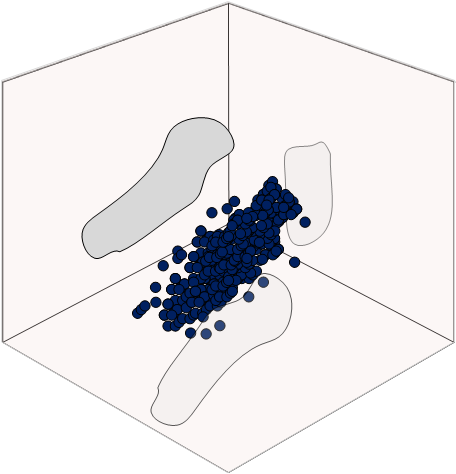
\includegraphics[scale=0.45]{IllustrationMatriceC2O.png}
    \caption{Color Contrast Occurence Matrix}\label{fig:Color Contrast Occurence Matrix}
\end{figure}

On the figure shown above, we can see an example of the cloud of points that we expect to obtain. There to thing which characterize the image :
\begin{itemize}
\item the size and the form of the cloud which characterize the texture around the keypoint.
\item the projections on the three plans of the representation which characterize the color information around the keypoint.
\end{itemize}
\paragraph{The Color Constrast Occurence feature}
~~\\
~~\\
With the cloud of point obtained by the computation of the Color Contrast Occurence matrix, we have a 3 dimensional representation of our keypoint. To reduce the quantity of data to store and to facilitate the distance calculation, we have to represent this matrix by at least a 2-dimensional feature.
To do that, the solution used is to realize a spherical quantization on the cloud of point to have a histogram which will represent our keypoint on two dimensions.
Each sphere will include a number of points of the cloud, but to have a better distribution, each sphere will be split in some part as shown below :

\begin{figure}[h]
    \center
    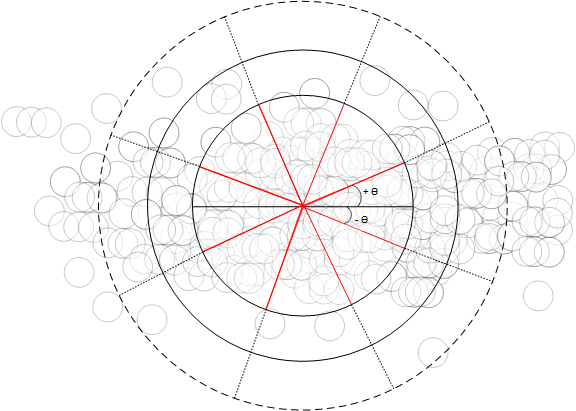
\includegraphics[scale=0.75]{QuantificationSpherique.png}
    \caption{Spheric quantizaton}\label{fig:Qantification sph�rique}
\end{figure}

Here we can see a sectionnal view of our spherical quantization. Each sphere is divided by n parts as show above, and the number of points in each part are concatenates one by one in the description vector (quarter after quarter and sphere after sphere).
% ----------------------------------------------------------------
\end{document} 